\documentclass[xetex,mathserif,serif]{beamer}
\usepackage{polyglossia}
\setdefaultlanguage[babelshorthands=true]{russian}
\usepackage{minted}
\usepackage{tabu}
\usepackage{moresize}

\useoutertheme{infolines}

\usepackage{fontspec}
\setmainfont{FreeSans}
\newfontfamily{\russianfonttt}{FreeSans}

\definecolor{links}{HTML}{2A1B81}
\hypersetup{colorlinks,linkcolor=,urlcolor=links}

\setbeamertemplate{blocks}[rounded][shadow=false]

\setbeamercolor*{block title alerted}{fg=red!50!black,bg=red!20}
\setbeamercolor*{block body alerted}{fg=black,bg=red!10}

\tabulinesep=1.2mm

\title{Работа с сетью}
\subtitle{Низкий уровень}
\author[Юрий Литвинов]{Юрий Литвинов\\\small{\textcolor{gray}{yurii.litvinov@gmail.com}}}
\date{21.09.2018г}

\newcommand{\attribution}[1] {
\vspace{-5mm}\begin{flushright}\begin{scriptsize}\textcolor{gray}{\textcopyright\, #1}\end{scriptsize}\end{flushright}
}

\begin{document}

	\frame{\titlepage}

	\section{Архитектура сети}

	\begin{frame}
		\frametitle{Архитектура глобальной сети}
		\begin{center}
			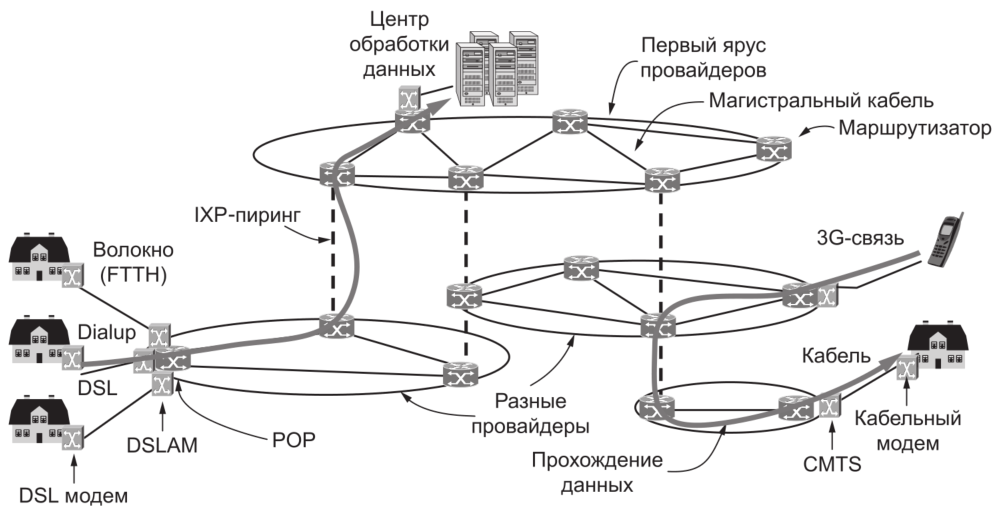
\includegraphics[width=0.9\textwidth]{internetArchitecture.png}
			\attribution{Э. Таненбаум}
		\end{center}
	\end{frame}

	\begin{frame}
		\frametitle{Уровневая архитектура}
		\framesubtitle{Модель OSI}
		\begin{center}
			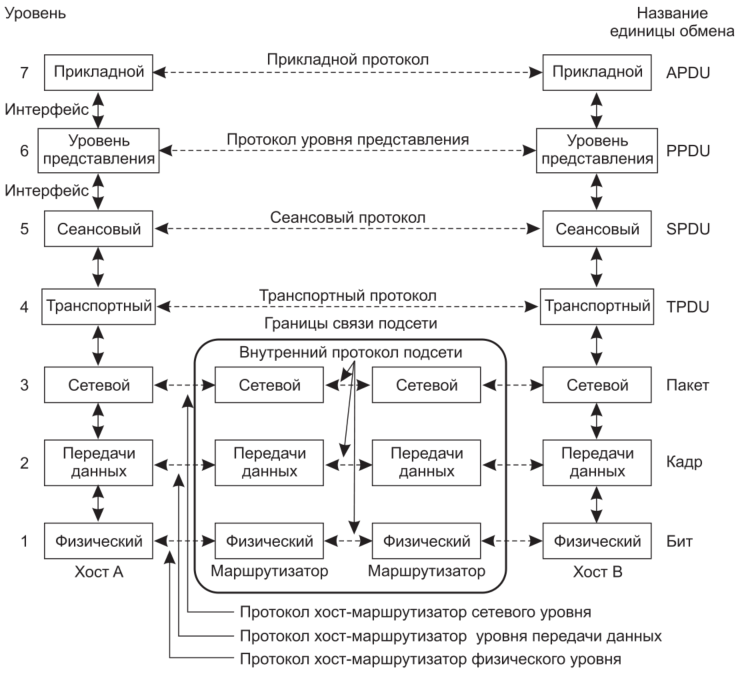
\includegraphics[width=0.6\textwidth]{osiStack.png}
			\attribution{Э. Таненбаум}
		\end{center}
	\end{frame}

	\begin{frame}
		\frametitle{Модель TCP/IP}
		\begin{center}
			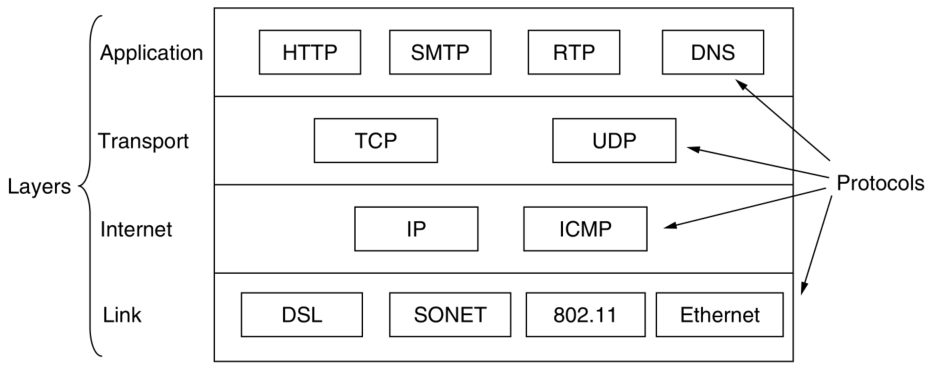
\includegraphics[width=0.9\textwidth]{tcpIpStack.png}
			\attribution{Э. Таненбаум}
		\end{center}
	\end{frame}

	\begin{frame}
		\frametitle{Физический уровень}
		\begin{itemize}
			\item Физические параметры канала (электрические, электромагнитные, ...)
			\item Ethernet (витая пара), USB, xDSL, Bluetooth, IEEE 802.11 (WiFi), оптические сети, спутниковая связь, мобильные сети (GSM, EDGE, LTE) и т.д.
			\begin{itemize}
				\item RFC 1149 ``IP over Avian Carriers'' (\url{https://tools.ietf.org/html/rfc1149})
			\end{itemize}
			\item Отвечает только за передачу сигнала в рамках среды распространения между двумя точками
			\item Вопросы кодирования битов уровнями сигнала, синхронизации, помехоустойчивости, мультиплексирования
			\item Передаёт биты или блоки битов
		\end{itemize}
	\end{frame}

	\begin{frame}
		\frametitle{Канальный уровень}
		\begin{itemize}
			\item Общение напрямую соединённых устройств сети
			\item PPP (Point to Point Protocol)
			\item Понятия MAC и LLC
			\item Вопросы коррекции ошибок физического уровня (коды Хэмминга, Рида-Соломона, свёрточные коды и прочая алгебра с теорией чисел), повтора передачи пропавших данных, управления скоростью передачи
			\item Передаёт фрэймы (или кадры)
		\end{itemize}
	\end{frame}

	\begin{frame}
		\frametitle{Сетевой уровень}
		\begin{itemize}
			\item Сеть из нескольких устройств
			\item Вопросы поиска оптимального маршрута внутри сети (роутинга), передачи по принципиально разным сетям (например, один пакет по оптоволокну, второй --- через спутник)
			\item IP (Internet Protocol)
			\item Понятие IP-адреса (IPv4, IPv6)
			\item Передаёт пакеты
		\end{itemize}
	\end{frame}

	\begin{frame}
		\frametitle{Транспортный уровень}
		\begin{itemize}
			\item Соединение двух устройств через сеть
			\item Вопросы надёжности доставки, разделения-сборки сообщения, правильного порядка сообщений, подтверждения и повторной отправки
			\item Протоколы TCP, UDP
			\begin{itemize}
				\item TCP --- протокол, гарантирующий доставку данных в правильном порядке, без потерь и порчи, если это вообще возможно
				\begin{itemize}
					\item Передача файлов, текстовых данных (включая веб-страницы), веб-сервисы
				\end{itemize}
				\item UDP --- протокол, позволяющий отправлять ``датаграммы'' без гарантий их доставки или доставки в правильном порядке, но в разы быстрее TCP
				\begin{itemize}
					\item Стриминг фильмов, музыки, компьютерные игры
				\end{itemize}
			\end{itemize}
		\end{itemize}
	\end{frame}

	\begin{frame}
		\frametitle{Сеансовый уровень}
		\begin{itemize}
			\item Установление, поддержание и закрытие соединения
			\item Протокол TCP
		\end{itemize}
	\end{frame}

	\begin{frame}
		\frametitle{Уровень представления}
		\begin{itemize}
			\item Кодировка и представление передаваемых данных
			\begin{itemize}
				\item Шифрование
				\item Сериализация/десериализация
			\end{itemize}
		\end{itemize}
	\end{frame}

	\begin{frame}
		\frametitle{Прикладной уровень}
		\begin{itemize}
			\item Общение конкретных приложений
			\item Протоколы HTTP, FTP, SMTP и т.д.
			\item Протоколы поверх HTTP: REST, SOAP и т.д.
		\end{itemize}
	\end{frame}

	\begin{frame}
		\frametitle{Порты и сокеты}
		\begin{itemize}
			\item Порт --- число от 1 до 65535
			\item Привязан к сетевому интерфейсу
			\item Ресурс, управляемый ОС
			\item Типичные порты
			\begin{itemize}
				\item 22 --- SSH
				\item 25 --- SMTP
				\item 80 --- HTTP
				\item 443 --- HTTPS
				\item 666 --- Doom
			\end{itemize}
			\item Сокет --- программный интерфейс к порту
			\item Сетевой стек --- важная часть операционной системы, сокеты --- способ для прикладного программиста с ним работать
		\end{itemize}
	\end{frame}

\end{document}
